\section{Koncepcje związane z projektowanym systemem}
\label{sec:Koncepcje związane z projektowanym systemem}

W ramach pracy wykonano system służący do wspomagania zarządzania czasem. Wybór tematu przykłdowej implementacji dyktowany jest możliwością zastosowania technik mikroprocesorowych i koncepcji IoT (Internet of Things) oraz możliwością porównania z podobnymi rozwiązaniami. Aplikacje tego typu są tworzone z myślą o wykonawcy zleceń, jak i o organizatorach. Zasadą ich działania jest zbieranie informacji od użytkownika dotyczące niezbędnych do wykonania zadań oraz układanie ich w formie planu - terminarza. W użyciu przypominają rozbudowany kalendarz umożliwiający łatwe dodawanie nowych zadań oraz podpowiadającego efektywne zagospodarowanie czasu.

\subsection{Model systemu rozproszonego}
\label{subs:Model systemu rozproszonego}

Koncepcja Internet of Things, w uproszczeniu sprowadza się do rozbudowaniu wszystkich urządzeń elektronicznych tak, by miały dostęp do Internetu. Komunikacja z urządzeniami poprzez sieć uznana za najważniejszą cechę urządzeń tworzonych wchodzących w skład takiego systemu. Często komunikacja oraz transfer danych bezpośrednio pomiędzy urządzeniem mobilnym, a komputerem PC, jest funkcją, która nie jest implementowana, ponieważ jest uznanawana za nadmiarową \cite{bib:iot-middleware}. Aby taki system mógł funkcjonować należy zapewnić możliwość nawiązania połączenia, poprawnej transmisji danych, oraz dostępu do serwera, który będzie pełnił rolę węzła głównego. Schemat rozwiązania znajduje się na rysunku \ref{figure:sys_synchro}.
\begin{figure}[ht]
  \centering
  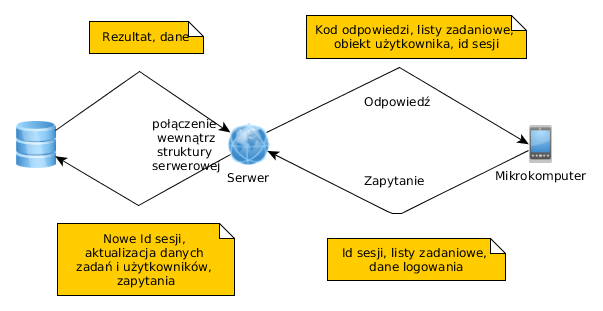
\includegraphics[width=\textwidth]{images/synchro.png}
  \caption{Schemat modelu komunikacji i wymiany danych}
  \label{figure:sys_synchro}
\end{figure}
\FloatBarrier

\subsection{Platforma mikroprocesorowa}

Na rynku istnieje wiele platform umożliwiających wykonanie zakładanego projektu. Lista takich urządzeń znajduje się na rysunku \ref{figure:hard_comparison}. Według kategoryzacji sugerowanej w pracy \cite{bib:mobile-paradigm}, przyjęto , że plaformami użytecznymi z punktu widzenia projektu będą te, które wspierają wieloprogramowość i obsługę wielu procesów. Te zadania pełni system operacyjny. Do celów implementacji rozwiązania wykożystano mikrokomputer Raspberry Pi B, ponieważ jest szeroko dostępny na polskim rynku, posiada wiele gotowych podzespołów do rozbudowy, jest dobrze wspierany przez producenta, ma możliwość zainstalowania systemu operacyjnego, posiada wystarczającą ilość pamięci RAM oraz wystarczająco szybko taktowany procesor, aby uruchomić system operacyjny wraz z graficzną aplikacją użytkownika. Gooseberry oraz Mars Board również spełniały wymagania techniczne, ale nie wymagały dodatkowej konfiguracji i dokupienia modułów zapewniających łączność z internetem i z urządzeniem peryferyjnym. Mikrokomputer BeagleBone Black oraz Raspberry Pi oferowały podobne funkcjonalności. O wyborze tego drugiego zadecydowała niższa cena rynkowa.

\begin{figure}[ht]
  \centering
  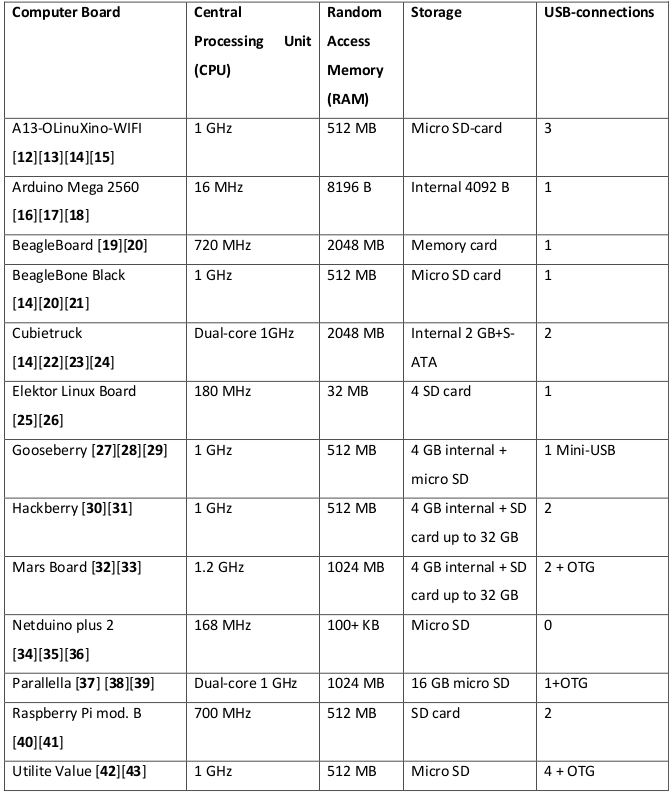
\includegraphics[width=0.95\textwidth]{images/hard_zestawienie.png}
  \caption{Zestawienie popularnych platform mikroprocesorowych\cite{bib:mgr-rpi}.}
  \label{figure:hard_comparison}
\end{figure}

Raspberry Pi w podstawowej konfiguracji sprzętowej posiada kartę sieciową wraz z interfejsem RJ45 zgodnym z technologią Fast Ethernet. Obsługa warstwy fizycznej odbywa się w module “LAN9514” firmy Microchip, który jest zintegrowany z czterema portami USB 2.0. Komunikacja procesora z modułem opiera się magistrali USB co narzuca ograniczenie technologiczne dotyczące prędkości przeysłu danych. Port obsługuje komunikaty sterowane za pomocą napięć (np. Wake On Lan, Zmiana statusu połączenia, “Magic Packet”). Wszystkie peryferia mikrokomputera działają w trybie serwera, łącze micro-usb służy wyłącznie do zasilania. Komunikacja z urządzeniem odbywa się na tej samej zasadzie co z innym komputerem stacjonarnym.

Nawiązanie połączenia komputer stacjnorany - mikrokomputer odbywać się może poprzez sieć lokalną, lub po odpowiednim skonfigurowaniu, poprzez internet. Podczas wykonywania zadania projektowego wykorzystywano bezpośrednie połączenie lokalne. System operacyjny dostarczony razem z urządzeniem zawiera niezbędne sterowniki, wspiera protokół dynamicznego przydzielania adresu (DHCP) oraz protokół zdalego logowania z szyfrowaniem (SSH). Dodatkowo, w celu uzyskania dostępu do trybu graficznego zainstalowano program \textit{vncserver} oraz \textit{vncclient} odpowiednio na urządzeniu mobilnym i komputerze z którego nawiązywano połączenie.

Jak wspomniano wyżej, integralną częścią platformy jest system operacyjny. Raspberry Pi umożliwia zastosowanie dowolnego, o ile wpiera on jego architekturę systemu (ARM w wersji 6). W tabeli \ref{figure:linux_comparison} zostały zamieszczone wszystkie, które obsługują procesory ARM. Producent platformy mikroprocesorowej rozwija dedykowaną dystrybucję (Raspbian), która zawiera pełne wsparcie dla zainstalowanych na płytce urządzeń peryferyjnych, oraz część sterowników do modułów rozszerzeń. Ze względu na wsparcie dla wyświetlacza dotykowego, który rozszerza funkcjonalność implementowanego rozwiązania, oraz szerokie wsparcie dla społeczności użytkowników tej dystrybucji w internecie, autorzy projektu zadecydowali użyć jej do realizacji pracy.



\begin{figure}[ht]
  \centering
  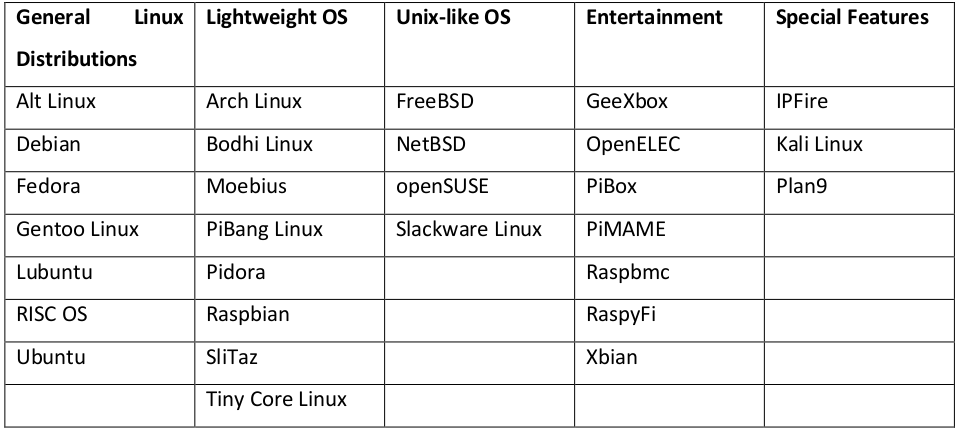
\includegraphics[width=\textwidth]{images/linux_zestawienie.png}
  \caption{Zestawienie systemów operacyjnych wspierających architekturę ARM\cite{bib:mgr-rpi}.}
  \label{figure:linux_comparison}
\end{figure}
\FloatBarrier

\section{Tworzenie interaktywnej aplikacji}
\label{subs:Narzędzia do wytwarzania oprogramowania}

Spośród dostępnych metod tworzenia aplikacji, których przeznaczeniem są platformy mobilne \cite{bib:mobile-paradigm}, w kontekście jej użycia jako elementu systemu wbudowanego możliwe do wdrożenia są: aplikacje pisane w kodzie natywnym danego urządzenia (w przypadku systemu Linux, byłby to język C++), przy wykorzystaniu niezależnego od platformy środowiska uruchomieniowego (Java/Python) lub przy wykorzystaniu technologii webowych.

Chcąc zachować elastyczność kodu i oraz zapewnić niezależność działania aplikacji od platformy i konfiguracji sprzętowej urządzenia na którym jest uruchamiana, aplikacja powinna zostać napisana w środowisku innym niż natywne. Z punktu widzenia przeznaczenia aplikacji - środowiska, w którym ważną rolę odgrywa ekran dotykowy - wybrane narzędzie programistyczne powinno wspierać i obsługiwać gesty wykonywane przez użytkownika w sposób jednolity i prosty, tak by umożliwić programiście skupienie się na logice wytwarzanej aplikacji. Zestawem bibliotek wspomagających wytwarzanie aplikacji w trybie graficznym obsługującym wiele zdarzeń - gestów jednocześnie, jest Kivy, PyQt dla języka Python oraz JavaFX i MT4j dla języka Java,

Do wytwarzania oprogramowania na platformę mobilną wykorzystano język Python. Jest to język, który jest aktualnie najbardziej popularnym wśród użytkowników mikrokomputerów, ze względu na prostotę składni i zachowanie wysokiej elastyczności kodu i możliwości rozbudowy aplikacji. Jako zestaw narzędzi wspomagających tworzenie aplikacji graficznej wybrano Kivy, ponieważ w odróżnieniu od PyQt zawiera wsparcie dla komunikacji sieciowej, oraz własny język (\textit{kv}) opisu elementów widoku (\textit{widgetów}).

Synchronizacja z aplikacją webową odbywa się przy użyciu zapytań RESTowych. Zapytania RESTowe, to odpowiednie zapytania protokołu HTTP, takie jak GET, POST, PUT, DELETE, które umożliwiają manipulację danymi. Za ich pomocą wykonywane są akcje tworzenia, czytania, modyfikacji i usuwania (ang. \textit{CRUD - Create, Read, Update and Delete}). Kivy dostarcza moduł zwany  UrlRequest, działający na podobnej zasadzie co funkcje zarządzające obiektami typu XHR\cite{bib:xhr} w języku JavaScript. UrlRequest obsługuje zapytania asynchroniczne. Oznacza to, że komunikacja sieciowa obsługiwana jest w osobnym wątku; główny powinien pozostać w stanie nie zablokowanym, ponieważ wykonuje on operacje aplikacji graficznej aplikacji graficznej, niezbędne do generowania widoku i utrzymania interakcji z uzytkownikiem. Po otrzymaniu wyniku, moduł UrlRequest wykonuje zdefiniowaną w jego parametrach metodę sygnalizującą program główny o rezultacie zapytania.

Aplikacja, której celem jest gromadzenie informacji o zadaniach użytkownika musi posiadać stukturę danych. Można taką strukturę tworzyć samodzielnie w postaci struktur danych i odpowiednio powiązanych klas, oraz opisać mechanizmy manipuluacji danymi umożliwiające zapis i odczyt tych struktur w plikach. Współcześnie istnieją rozwiązania zaczerpnięte z technologii webowej, które ułatwiają tworzenie, systematyzację i przechowywanie danych. Do najpopularniejszych należą ORM (\textit{Object-relational mapping}) oraz SQL-Speaking Objects. W swoim działaniu opierają się na relacyjnych bazach danych, posiadają mechanizmy zapewniające spójność danych oraz wbudowane mechanizmy zabezpieczające przed przypadkowym i szkodliwym działaniem czynników niezależnych od algorytmu podczas operacji zapisu/odczytu danych do własnej bazy danych. Dzięki tego typu rozwiązaniu, programista ma zapewniony dostęp do pliku przechowującego dane na zewnątrz aplikacji, które nie znikną po jego zamknięciu, oraz ma pewność co do poprawności i kompletności operacji na nim wykonywanych. Podczas implementacji aplikacji do zarządzania zadaniami wykorzystano ORM dedykowany językowi Python: \textit{SQLAlchemy}.


\begin{figure}[ht]
  \centering
  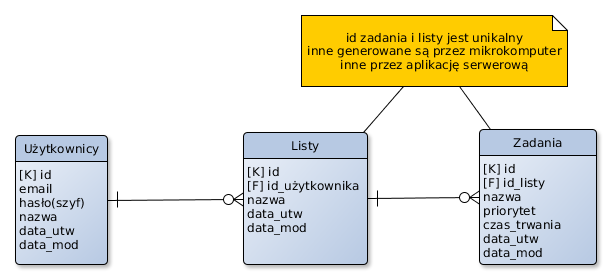
\includegraphics[width=\textwidth]{images/dane.png}
  \caption{Uproszczony model bazy danych. Symbol [K] oznacza klucz podstawowy, [F] oznacza klucz obcy.}
  \label{figure:dane}
\end{figure}

Baza danych aplikacji w uproszczeniu wygląda tak jak przedstawiono na rysunku \ref{figure:dane}.

Zestawienie narzędzi oraz technologii używanej przy tworzeniu aplikacji mobilnej:
Instalacja i konfiguracja systemu operacyjnego:
\begin{itemize}
  \item Raspbian - dystrybucja Linuxa
  \item LXDE - środowisko graficzne
\end{itemize}

Środowisko tworzenia aplikacji:
\begin{itemize}
  \item Język - Python, wersja 2.7
  \item Interfejs użytkownika - Kivy
  \item Obsługa zapytań RESTowych - Kivy
  \item Implementacja modelu bazy danych (ORM) - SqlAlchemy
\end{itemize}

\begin{figure}[ht]
  \centering
  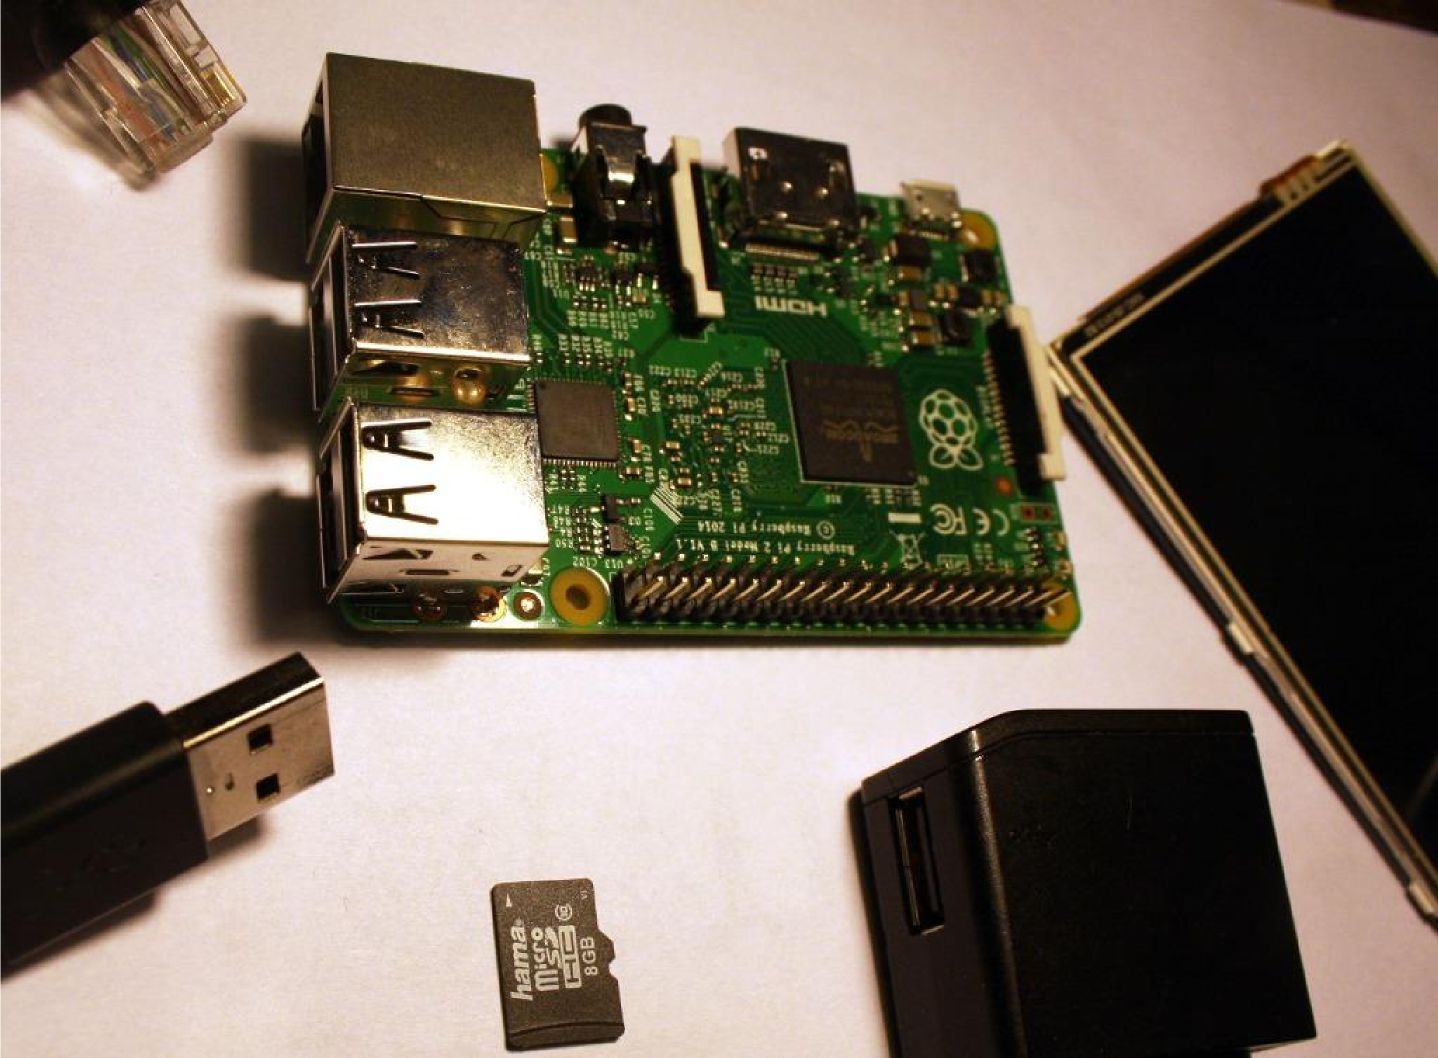
\includegraphics[width=\textwidth]{images/konfiguracja.png}
  \caption{Konfiguracja systemu: mikrokomputer, pamięć, zasilanie, wyświetlacz i medium transmisyjne
}
  \label{figure:konfig}
\end{figure}


\section{Aplikacja serwerowa}

Do zaimplementowania aplikacji serwerowej wykorzystaliśmy:

\begin{itemize}
  \item język programowania Ruby, versja 2.2.2 \cite{bib:ruby-doc}
  \item Framework Ruby on Rails, versja 4.2.3 \cite{bib:rails-doc}
  \item CoffeScript \cite{bib:coffeescript-doc}
  \item Sass \cite{bib:sass-doc}
  \item Bibliotekę jQuery do języka javaScript \cite{bib:jquery-doc}
  \item Bazę danych SQLlite
\end{itemize}

Wybór padł na technologię Ruby on Rails głównie ze względu na łatwość integracji z REST-owym API, ale ważnymi czynnikami były także: szybkość powstawania aplikacji internetowych w tym frameworku, oraz na obecną popularność na rynku.

\subsection {Instalacja i uruchomienie aplikacji serwerowej}

Aby uruchomić środowisko aplikacji, należy mieć zainstalowany język ruby oraz framework Ruby on Rails, wraz ze wszystkimi potrzebnymi wtyczkami. W systemie Ubutntu, aby to osiągnąć, należy najpierw zainstalować manager wersji Ruby (RVM \cite{bib:rvm-install}). Kiedy mamy to zrobione, należy uruchomić terminal, jprzejść do folderu aplikacji, a następnie zainstalować wersję 2.2.2 języka Ruby oraz odpowiedni komplet gemów.

\begin{lstlisting}
  rvm install 2.2.2
  rvm use 2.2.2@test --create
  gem install bundler
  bundle install
\end{lstlisting}


Po zakończeniu wykonywania powyższych komend, śodowisko aplikacji powinno być zainstalowane. Kolejnym krokiem jest uruchomienie lokalnego serwera aplikacji.

\begin{lstlisting}
  rails s
\end{lstlisting}

Od tej pory aplikacja powinna być dostępna pod adresem \url{http://localhost:3000}, co widać na rysunku \ref{figure:root-page-server},

\begin{figure}[ht]
  \centering
  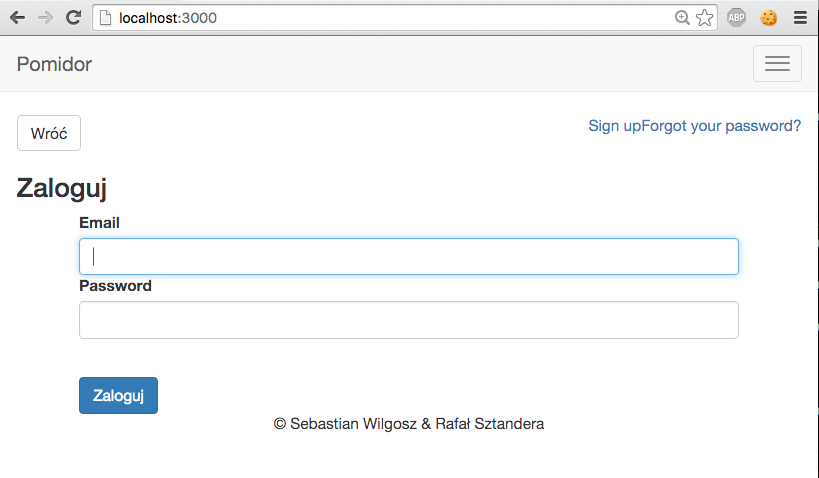
\includegraphics[scale=0.35]{images/root-page-server.png}
  \caption{Widok strony głównej aplikacji}
  \label{figure:root-page-server}
\end{figure}
\FloatBarrier
